\let\negmedspace\undefined
\let\negthickspace\undefined
\documentclass[journal,12pt,onecolumn]{IEEEtran}
\usepackage{cite}
\usepackage{amsmath,amssymb,amsfonts,amsthm}
\usepackage{algorithmic}
\usepackage{graphicx}
\graphicspath{{./figs/}}
\usepackage{textcomp}
\usepackage{xcolor}
\usepackage{txfonts}
\usepackage{listings}
\usepackage{enumitem}
\usepackage{mathtools}
\usepackage{gensymb}
\usepackage{comment}
\usepackage{caption}
\usepackage[breaklinks=true]{hyperref}
\usepackage{tkz-euclide} 
\usepackage{listings}
\usepackage{gvv}                                        
%\def\inputGnumericTable{}                                 
\usepackage[latin1]{inputenc}     
\usepackage{xparse}
\usepackage{color}                                            
\usepackage{array}
\usepackage{longtable}                                       
\usepackage{calc}                                             
\usepackage{multirow}
\usepackage{multicol}
\usepackage{hhline}                                           
\usepackage{ifthen}                                           
\usepackage{lscape}
\usepackage{tabularx}
\usepackage{array}
\usepackage{float}
\newtheorem{theorem}{Theorem}[section]
\newtheorem{problem}{Problem}
\newtheorem{proposition}{Proposition}[section]
\newtheorem{lemma}{Lemma}[section]
\newtheorem{corollary}[theorem]{Corollary}
\newtheorem{example}{Example}[section]
\newtheorem{definition}[problem]{Definition}
\newcommand{\BEQA}{\begin{eqnarray}}
\newcommand{\EEQA}{\end{eqnarray}}
\newcommand{\define}{\stackrel{\triangle}{=}}
\theoremstyle{remark}
\newtheorem{rem}{Remark}

\begin{document}

\title{5.9.10}
\author{ee25btech11056 - Suraj.N}
\maketitle
\renewcommand{\thefigure}{\theenumi}
\renewcommand{\thetable}{\theenumi}

\begin{document}

\textbf{Question :} A fraction becomes $\tfrac{1}{3}$ when $2$ is subtracted from the numerator and it becomes $\tfrac{1}{2}$ when $1$ is subtracted from the denominator. Find the fraction.

\textbf{Solution :} 

\begin{table}[h!]
  \centering
  \begin{table}[h!]
    \centering
    \begin{tabular}{|c|c|}
        \hline
        Point & Coordinates \\
        \hline
	    $A$ & $\myvec{1\\-1}$ \\
	    $B$ & $\myvec{-4\\2k}$ \\
	    $C$ & $\myvec{-k\\-5}$ \\
        \hline
    \end{tabular}
    \caption{Vertices of $\triangle ABC$ before substituting $k$}
    \label{tab:triangle_k}
\end{table}

  \caption*{Table : Equations}
  \label{5.9.10}
\end{table}

Let the fraction be $\dfrac{x}{y}$ , using the given conditions we get ,

\begin{align}
  \dfrac{x-2}{y} &= \dfrac{1}{3}\\
  3x - y &= 6\\
  \dfrac{x}{y-1} &= \dfrac{1}{2}\\
  2x - y &= -1
\end{align}

The system of equations formed is :

\begin{align}
3x - y &= 6\\
2x - y &= -1
\end{align}

Writing it in the matrix form,

\begin{align}
  \myvec{3 & -1\\2 & -1}\myvec{x\\y} &= \myvec{6\\-1}
\end{align}

Forming the augmented matrix to solve the system of equations,

\begin{align}
  \myaugvec{2}{3 & -1 & 6\\2 & -1 & -1}
\end{align}

Using Gaussian Elimination,

\begin{align}
 \myaugvec{2}{3 & -1 & 6\\2 & -1 & -1} 
 \xleftrightarrow{\;R_2 \to R_2 -\tfrac{2}{3}R_1}
 \myaugvec{2}{3 & -1 & 6\\0 & -\tfrac{1}{3} & -5} 
\end{align}

Using back substitution we get,

\begin{align}
  -\tfrac{y}{3} &= -5\\
  y &= 15\\
3x-y &= 6\\
  3x &= 6 + 15\\
  x &= 7
\end{align}

\pagebreak 

The solution for the system of equations is :

\begin{align}
  \myvec{x\\y} &= \myvec{7\\15}
\end{align}

Therefore the fraction is 

\begin{align}
  \dfrac{x}{y} &= \dfrac{7}{15}
\end{align}

\pagebreak

\begin{figure}[h!]
  \centering
  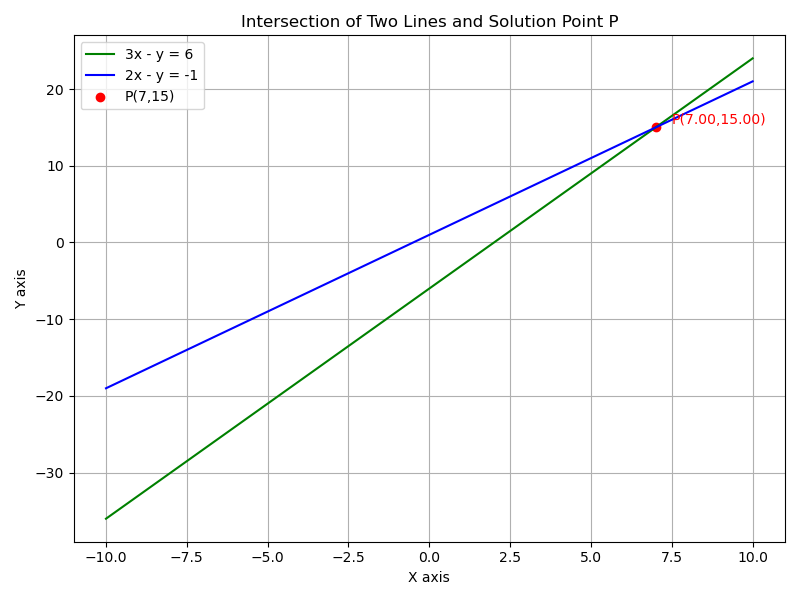
\includegraphics[width=0.7\columnwidth]{figs/solution.png} 
   \caption*{Fig : Lines}
  \label{Fig1}
\end{figure}


\end{document}
